\documentclass[11pt,a4paper]{report}
\usepackage[textwidth=37em,vmargin=30mm]{geometry}
\usepackage{calc,xunicode,amsmath,amssymb,paralist,enumitem,tabu,booktabs,datetime2,xeCJK,xeCJKfntef,listings}
\usepackage{tocloft,fancyhdr,tcolorbox,xcolor,graphicx,eso-pic,xltxtra,xelatexemoji}

\newcommand{\envyear}[0]{2024}
\newcommand{\envdatestr}[0]{2024-10-17}
\newcommand{\envfinaldir}[0]{webdb/2024/20241017/final}

\usepackage[hidelinks]{hyperref}
\hypersetup{
    colorlinks=false,
    pdfpagemode=FullScreen,
    pdftitle={Web Digest - \envdatestr}
}

\setlength{\cftbeforechapskip}{10pt}
\renewcommand{\cftchapfont}{\rmfamily\bfseries\large\raggedright}
\setlength{\cftbeforesecskip}{2pt}
\renewcommand{\cftsecfont}{\sffamily\small\raggedright}

\setdefaultleftmargin{2em}{2em}{1em}{1em}{1em}{1em}

\usepackage{xeCJK,xeCJKfntef}
\xeCJKsetup{PunctStyle=plain,RubberPunctSkip=false,CJKglue=\strut\hskip 0pt plus 0.1em minus 0.05em,CJKecglue=\strut\hskip 0.22em plus 0.2em}
\XeTeXlinebreaklocale "zh"
\XeTeXlinebreakskip = 0pt


\setmainfont{Brygada 1918}
\setromanfont{Brygada 1918}
\setsansfont{IBM Plex Sans}
\setmonofont{JetBrains Mono NL}
\setCJKmainfont{Noto Serif CJK SC}
\setCJKromanfont{Noto Serif CJK SC}
\setCJKsansfont{Noto Sans CJK SC}
\setCJKmonofont{Noto Sans CJK SC}

\setlength{\parindent}{0pt}
\setlength{\parskip}{8pt}
\linespread{1.15}

\lstset{
	basicstyle=\ttfamily\footnotesize,
	numbersep=5pt,
	backgroundcolor=\color{black!5},
	showspaces=false,
	showstringspaces=false,
	showtabs=false,
	tabsize=2,
	captionpos=b,
	breaklines=true,
	breakatwhitespace=true,
	breakautoindent=true,
	linewidth=\textwidth
}






\newcommand{\coverpic}[2]{
    % argv: itemurl, authorname
    Cover photo by #2~~(\href{#1}{#1})
}
\newcommand{\makeheader}[0]{
    \begin{titlepage}
        % \newgeometry{hmargin=15mm,tmargin=21mm,bmargin=12mm}
        \begin{center}
            
            \rmfamily\scshape
            \fontspec{BaskervilleF}
            \fontspec{Old Standard}
            \fontsize{59pt}{70pt}\selectfont
            WEB\hfill DIGEST
            
            \vfill
            % \vskip 30pt
            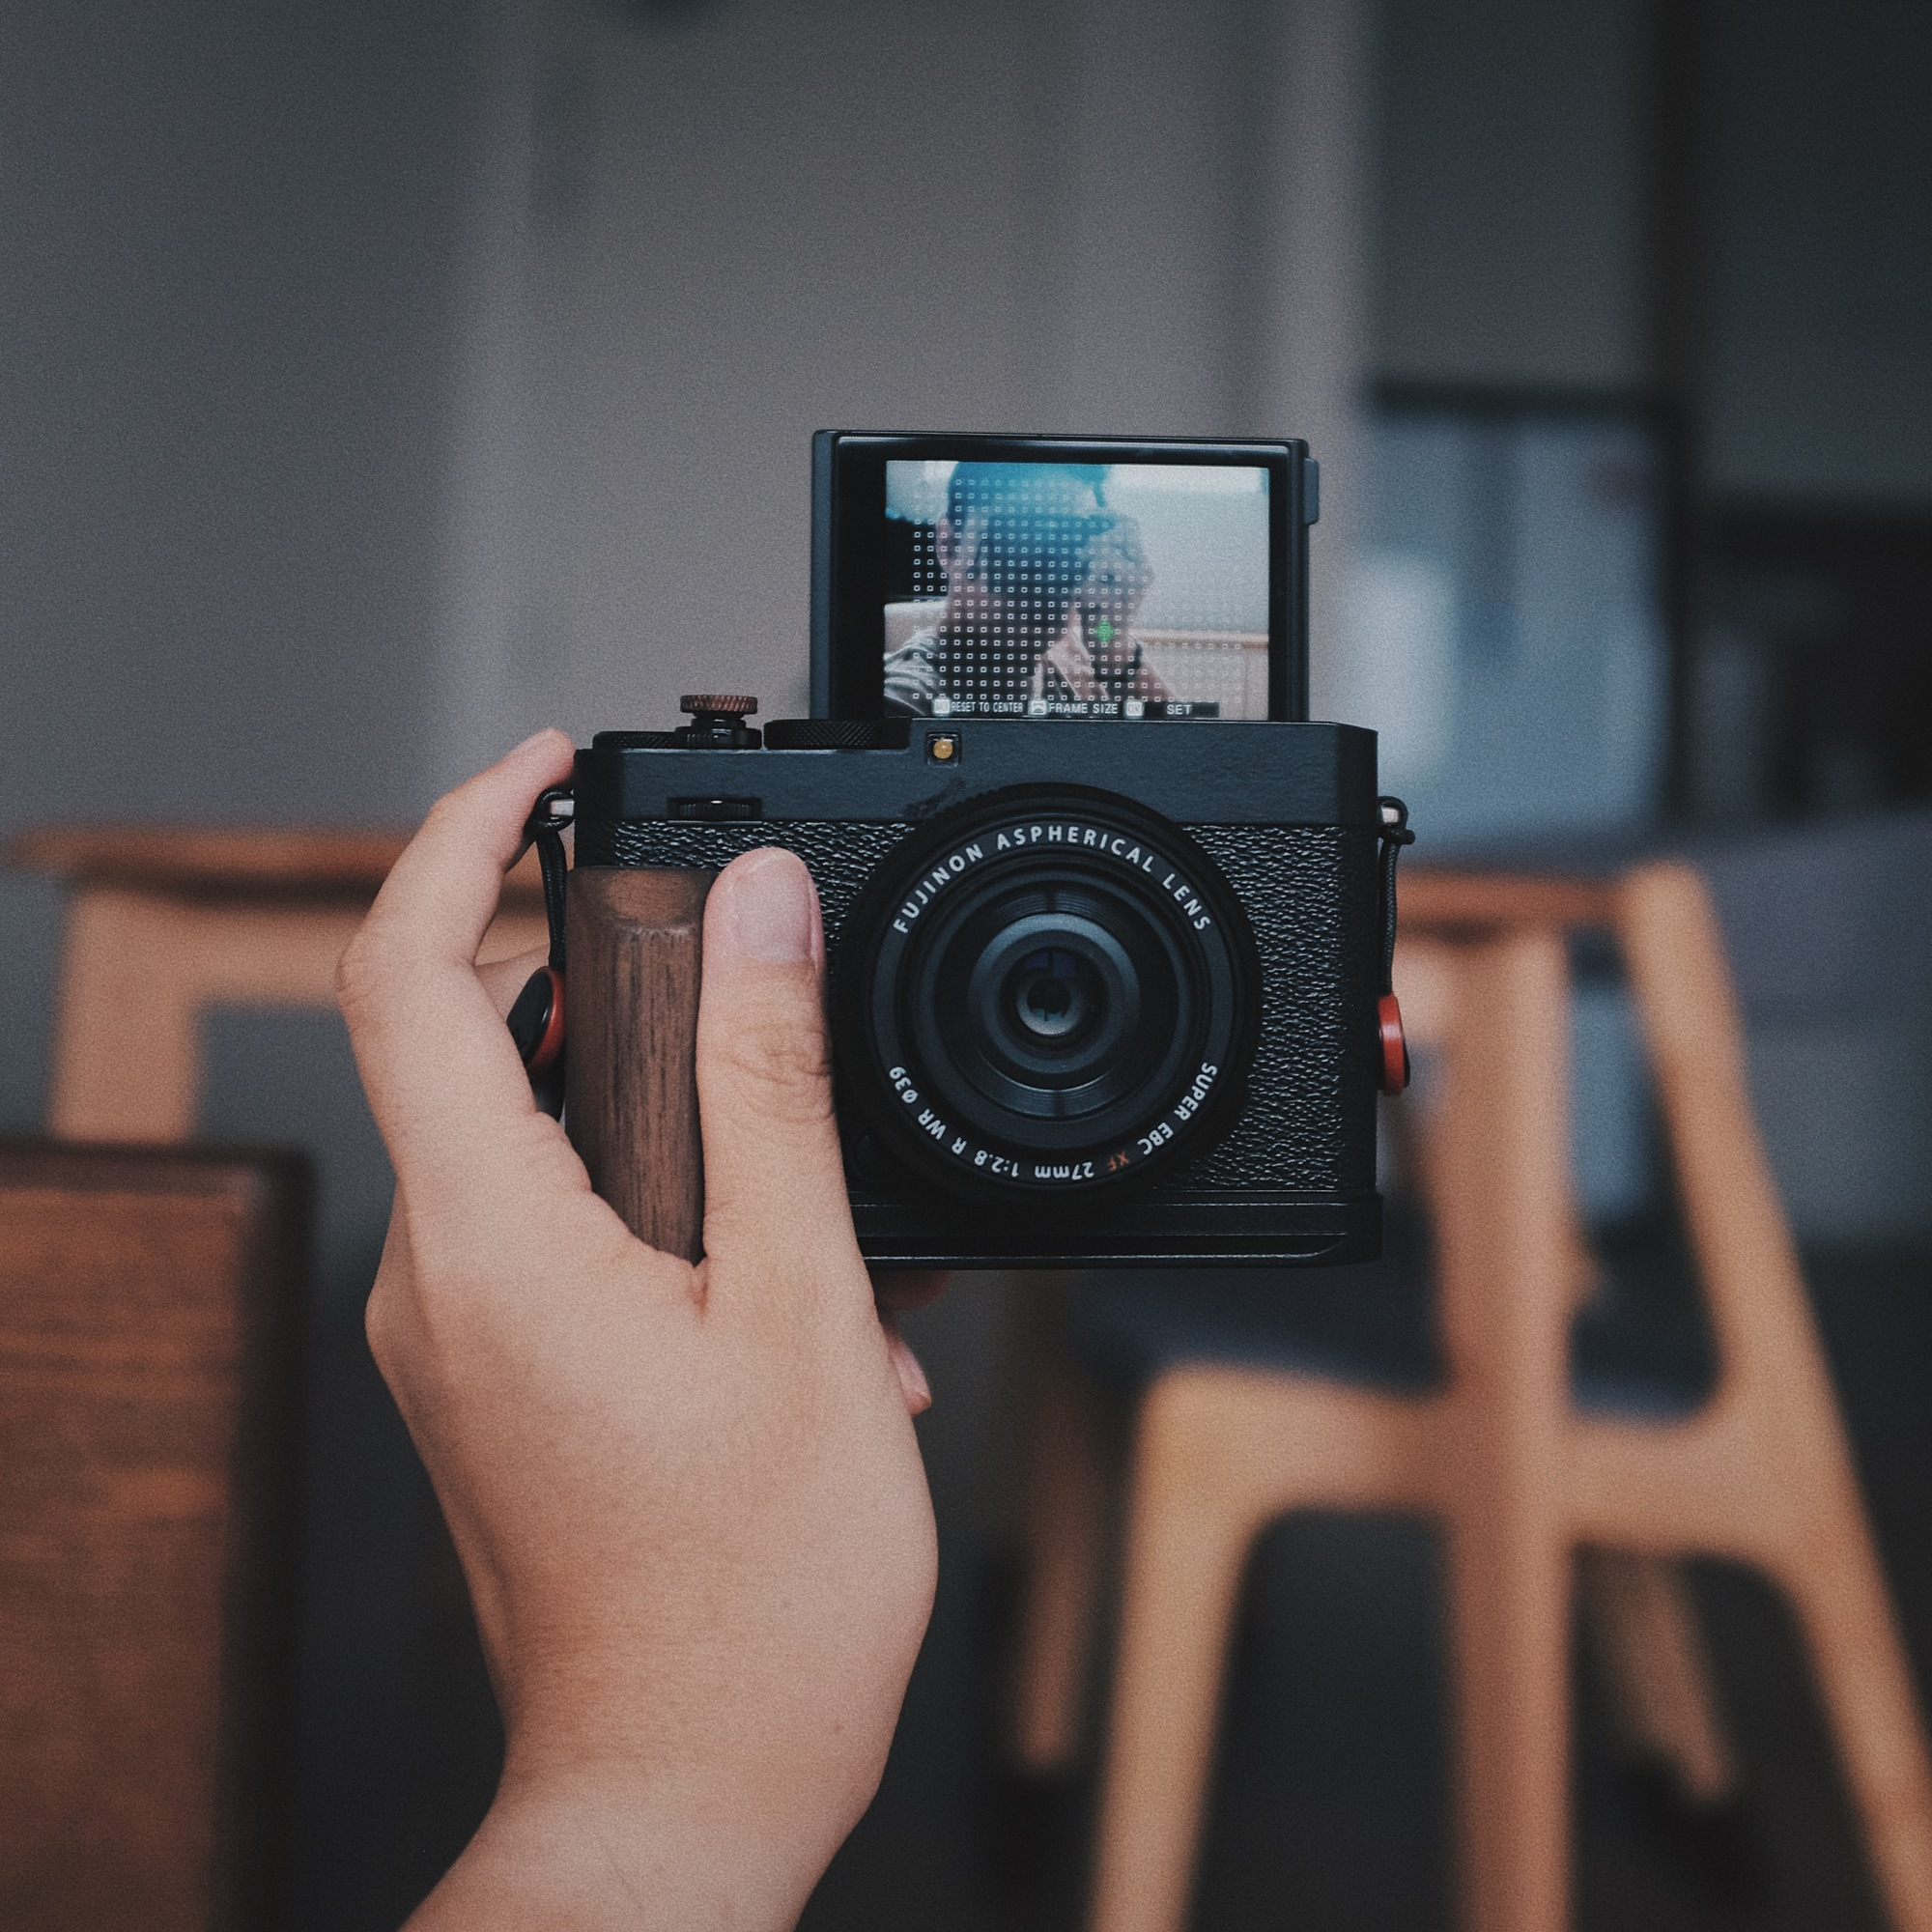
\includegraphics[width=\linewidth]{\envfinaldir/coverpic-prod.jpg}\par
            % \vskip 30pt
            \vfill

            \normalsize\rmfamily\scshape
            \copyright{} The Web Digest Project \hfill\large \envdatestr
        \end{center}
    \end{titlepage}
    % \restoregeometry
}
\newcommand{\simplehref}[1]{%
    \textcolor{blue!80!green}{\href{#1}{#1}}%
}
\renewcommand{\contentsname}{\center\Huge\sffamily\bfseries Contents\par\vskip 20pt}
\newcounter{ipartcounter}
\setcounter{ipartcounter}{0}
\newcommand{\ipart}[1]{
    % \vskip 20pt
    \clearpage
    \stepcounter{ipartcounter}
    \phantomsection
    \addcontentsline{toc}{chapter}{#1}
    % \begin{center}
    %     \Huge
    %     \sffamily\bfseries
    %     #1
    % \end{center}
    % \vskip 20pt plus 7pt
}
\newcounter{ichaptercounter}
\setcounter{ichaptercounter}{0}
\newcommand{\ichapter}[1]{
    % \vskip 20pt
    \clearpage
    \stepcounter{ichaptercounter}
    \phantomsection
    \addcontentsline{toc}{section}{\numberline{\arabic{ichaptercounter}}#1}
    \begin{center}
        \Huge
        \sffamily\bfseries
        #1
    \end{center}
    \vskip 20pt plus 7pt
}
\newcommand{\entrytitlefont}[1]{\subsection*{\raggedright\Large\sffamily\bfseries#1}}
\newcommand{\entryitemGeneric}[2]{
    % argv: title, url
    \parbox{\linewidth}{
        \entrytitlefont{#1}\par\vskip 5pt
        \footnotesize\ttfamily\mdseries
        \simplehref{#2}
    }\vskip 11pt plus 11pt minus 1pt
}
\newcommand{\entryitemGithub}[3]{
    % argv: title, url, desc
    \parbox{\linewidth}{
        \entrytitlefont{#1}\par\vskip 5pt
        \footnotesize\ttfamily\mdseries
        \simplehref{#2}\par\vskip 5pt
        \small\rmfamily\mdseries#3
    }\vskip 11pt plus 11pt minus 1pt
}
\newcommand{\entryitemAp}[3]{
    % argv: title, url, desc
    \parbox{\linewidth}{
        \entrytitlefont{#1}\par\vskip 5pt
        \footnotesize\ttfamily\mdseries
        \simplehref{#2}\par\vskip 5pt
        \small\rmfamily\mdseries#3
    }\vskip 11pt plus 11pt minus 1pt
}
\newcommand{\entryitemHackernews}[3]{
    % argv: title, hnurl, rawurl
    % \parbox{\linewidth}{
    %     \entrytitlefont{#1}\par\vskip 5pt
    %     \footnotesize\ttfamily\mdseries
    %     \simplehref{#3}\par
    %     \textcolor{black!50}{\href{#2}{#2}}
    % }\vskip 11pt plus 11pt minus 1pt
    \begin{minipage}{\linewidth}
            \entrytitlefont{#1}\par\vskip 5pt
            \footnotesize\ttfamily\mdseries
            \simplehref{#3}\par
            \textcolor{black!50}{\href{#2}{#2}}
    \end{minipage}\par\vskip 11pt plus 11pt minus 1pt
}







\begin{document}

\makeheader

\tableofcontents\clearpage




\ipart{Developers}
\ichapter{Hacker News}
\entryitemTwoLinks{AI PCs Aren't Good at AI: The CPU Beats the NPU}{https://news.ycombinator.com/item?id=41863061}{https://github.com/usefulsensors/qc\_npu\_benchmark}

\entryitemTwoLinks{We outsmarted CSGO cheaters with IdentityLogger}{https://news.ycombinator.com/item?id=41862028}{https://mobeigi.com/blog/gaming/how-we-outsmarted-csgo-cheaters-with-identitylogger/}

\entryitemTwoLinks{Ireland's big school secret: how a year off-curriculum changes teenage lives}{https://news.ycombinator.com/item?id=41861628}{https://www.theguardian.com/lifeandstyle/2024/oct/16/ireland-school-secret-transition-year-off-curriculum}

\entryitemTwoLinks{Winamp deletes entire GitHub source code repo after a rocky few weeks}{https://news.ycombinator.com/item?id=41861056}{https://arstechnica.com/gadgets/2024/10/winamp-really-whips-open-source-coders-into-frenzy-with-its-source-release/}

\entryitemTwoLinks{ArchiveBox is evolving: the future of self-hosted internet archives}{https://news.ycombinator.com/item?id=41860909}{https://docs.sweeting.me/s/archivebox-plugin-ecosystem-announcement}

\entryitemTwoLinks{It's not enough for a program to work – it has to work for the right reasons}{https://news.ycombinator.com/item?id=41860135}{https://buttondown.com/hillelwayne/archive/be-suspicious-of-success/}

\entryitemTwoLinks{Efficient high-resolution image synthesis with linear diffusion transformer}{https://news.ycombinator.com/item?id=41859805}{https://nvlabs.github.io/Sana/}

\entryitemTwoLinks{Un Ministral, Des Ministraux}{https://news.ycombinator.com/item?id=41859466}{https://mistral.ai/news/ministraux/}

\entryitemTwoLinks{Traveling with Apple Vision Pro}{https://news.ycombinator.com/item?id=41859012}{https://azadux.blog/2024/10/08/traveling-with-apple-vision-pro/}

\entryitemTwoLinks{Hofstadter on Lisp (1983)}{https://news.ycombinator.com/item?id=41858975}{https://gist.github.com/jackrusher/5139396}

\entryitemTwoLinks{Amazon buys stake in nuclear energy developer in push to power data centres}{https://news.ycombinator.com/item?id=41858863}{https://www.ft.com/content/00776191-b010-4104-add4-8dc430386911}

\entryitemTwoLinks{FTC announces "click-to-cancel" rule making it easier to cancel subscriptions}{https://news.ycombinator.com/item?id=41858665}{https://www.ftc.gov/news-events/news/press-releases/2024/10/federal-trade-commission-announces-final-click-cancel-rule-making-it-easier-consumers-end-recurring}

\entryitemTwoLinks{The Internet Archive is back online}{https://news.ycombinator.com/item?id=41857754}{https://arstechnica.com/tech-policy/2024/10/the-internet-archive-and-its-916-billion-saved-webpages-are-back-online/}

\entryitemTwoLinks{FLOSS/fund for free and open source projects}{https://news.ycombinator.com/item?id=41857032}{https://floss.fund/blog/announcing-floss-fund/}

\entryitemTwoLinks{MacOS sometimes leaks traffic after system updates}{https://news.ycombinator.com/item?id=41856883}{https://mullvad.net/en/blog/macos-sometimes-leaks-traffic-after-system-updates}

\entryitemTwoLinks{I Self-Hosted Llama 3.2 with Coolify on My Home Server}{https://news.ycombinator.com/item?id=41855886}{https://geek.sg/blog/how-i-self-hosted-llama-32-with-coolify-on-my-home-server-a-step-by-step-guide}

\entryitemTwoLinks{Let Google decide}{https://news.ycombinator.com/item?id=41855512}{https://cupofsquid.com/post/not-real/}

\entryitemTwoLinks{Medical student's apparent celiac disease responded to giardiasis treatment}{https://news.ycombinator.com/item?id=41855307}{https://www.backpacker.com/skills/outdoor-first-aid/are-those-stomach-troubles-celiac-or-giardia/}

\entryitemTwoLinks{Reflections on Palantir}{https://news.ycombinator.com/item?id=41855006}{https://nabeelqu.substack.com/p/reflections-on-palantir}

\entryitemTwoLinks{Eye Contact Correction: Redirecting the eyes to look at the camera}{https://news.ycombinator.com/item?id=41854801}{https://www.sievedata.com/functions/sieve/eye-contact-correction}\ichapter{Phoronix}
\entryitemGeneric{\hskip 0pt{}AMD Releases AOMP 20.0-0 For Radeon/Instinct Compiler Offloading}{https://www.phoronix.com/news/AMD-AOMP-20.0-0-Compiler}

\entryitemGeneric{\hskip 0pt{}Qualcomm Announces Mesa VCL Driver For OpenCL Acceleration Within VMs}{https://www.phoronix.com/news/Qualcomm-VCL-VirtIO-OpenCL}

\entryitemGeneric{\hskip 0pt{}Open-Source Radeon Vulkan Driver "RADV" Demonstrated On Windows}{https://www.phoronix.com/news/RADV-Windows-XDC-2024}

\entryitemGeneric{\hskip 0pt{}Intel Lunar Lake vs. AMD Strix Point Platform Profile Performance Comparison}{https://www.phoronix.com/review/lunar-lake-profiles}

\entryitemGeneric{\hskip 0pt{}GCC Preparing To Set C23 "GNU23" As Default C Language Version}{https://www.phoronix.com/news/GCC-Prepares-std-gnu23-Default}

\entryitemGeneric{\hskip 0pt{}Red Hat Enterprise Linux AI 1.2 Brings AMD ROCm + Instinct Tech Preview}{https://www.phoronix.com/news/Red-Hat-RHEL-AI-1.2}

\entryitemGeneric{\hskip 0pt{}AMD Linux Graphics Driver To Switch To More Aggressive Power Heuristics By Default}{https://www.phoronix.com/news/AMDGPU-More-Aggressive-Power}

\entryitemGeneric{\hskip 0pt{}Intel Low Power Mode Daemon v0.0.8 Brings New Features}{https://www.phoronix.com/news/Intel-Low-Power-LPMD-0.0.8}

\entryitemGeneric{\hskip 0pt{}New Patches Allow For Deleting Files ~54\% Faster On F2FS}{https://www.phoronix.com/news/F2FS-Faster-Truncate-Delete}


\ipart{Developers~~~~(zh-Hans)}
\ichapter{Solidot}
\entryitemGeneric{\hskip 0pt{}突触变化将多次获胜的小鼠变成恶霸}{https://www.solidot.org/story?sid=79509}

\entryitemGeneric{\hskip 0pt{}三季度智能手机出货量增长 4\%}{https://www.solidot.org/story?sid=79508}

\entryitemGeneric{\hskip 0pt{}青少年社媒使用与焦虑和抑郁强相关}{https://www.solidot.org/story?sid=79507}

\entryitemGeneric{\hskip 0pt{}日本继续工作的 65 岁以上老年人数量超 900 万}{https://www.solidot.org/story?sid=79506}

\entryitemGeneric{\hskip 0pt{}日本高滨核电站 1 号机组获准运行超过 50 年}{https://www.solidot.org/story?sid=79505}

\entryitemGeneric{\hskip 0pt{}太阳活动进入极大期}{https://www.solidot.org/story?sid=79504}

\entryitemGeneric{\hskip 0pt{}Google Chrome 开始自动禁用 uBlock Origin}{https://www.solidot.org/story?sid=79503}

\entryitemGeneric{\hskip 0pt{}诺贝尔经济学奖授予了证明制度对国家繁荣重要性的三位经济学家}{https://www.solidot.org/story?sid=79502}

\entryitemGeneric{\hskip 0pt{}AMD 和英特尔宣布在 x86 架构实现上展开合作}{https://www.solidot.org/story?sid=79501}

\entryitemGeneric{\hskip 0pt{}硅谷高管 Bob Lee 遇刺案本周开始审讯}{https://www.solidot.org/story?sid=79500}

\entryitemGeneric{\hskip 0pt{}将 Android 手机变成监听工具}{https://www.solidot.org/story?sid=79499}

\entryitemGeneric{\hskip 0pt{}英国考虑将 USB-C 作为通用充电端口}{https://www.solidot.org/story?sid=79498}

\entryitemGeneric{\hskip 0pt{}BBS 共同发明人 Ward Christensen 去世,享年 78 岁}{https://www.solidot.org/story?sid=79497}

\entryitemGeneric{\hskip 0pt{}Windows 10 将在一年后终止支持}{https://www.solidot.org/story?sid=79496}

\entryitemGeneric{\hskip 0pt{}WordPress 禁止 WP Engine 赞助和参与 WordPress 用户活动}{https://www.solidot.org/story?sid=79495}

\entryitemGeneric{\hskip 0pt{}赞比亚面临气候引起的能源危机}{https://www.solidot.org/story?sid=79494}

\entryitemGeneric{\hskip 0pt{}国家计算机病毒应急处理中心反驳伏特台风}{https://www.solidot.org/story?sid=79493}

\entryitemGeneric{\hskip 0pt{}Inkscape 1.4 释出}{https://www.solidot.org/story?sid=79492}

\entryitemGeneric{\hskip 0pt{}特斯拉 Optimus 机器人在活动上由人类远程控制}{https://www.solidot.org/story?sid=79491}

\entryitemGeneric{\hskip 0pt{}互联网档案馆以只读模式恢复上线}{https://www.solidot.org/story?sid=79490}\ichapter{V2EX}
\entryitemGeneric{\hskip 0pt{}[问与答] Follow 可以直接查看原文吗?还是同样需要跳转到源站查看?}{https://www.v2ex.com/t/1081011}

\entryitemGeneric{\hskip 0pt{}[Microsoft Office] 微软的大杀器 pbi 怎么不在 mac 平台推出呢?}{https://www.v2ex.com/t/1081010}

\entryitemGeneric{\hskip 0pt{}[宽带症候群] 机场支付宝的支付有没有风险的?}{https://www.v2ex.com/t/1081009}

\entryitemGeneric{\hskip 0pt{}[iPhone] 用大功率充电头会导致电池健康严重减少?}{https://www.v2ex.com/t/1081008}

\entryitemGeneric{\hskip 0pt{}[宽带症候群] 上海电信上传限速临时解决方案?}{https://www.v2ex.com/t/1081007}

\entryitemGeneric{\hskip 0pt{}[宽带症候群] 猫棒淘汰出来了,还有其他作用吗}{https://www.v2ex.com/t/1081005}

\entryitemGeneric{\hskip 0pt{}[服务器] 有没有比较干净整体迁移服务器上所有服务的软件或者系统。}{https://www.v2ex.com/t/1081004}

\entryitemGeneric{\hskip 0pt{}[路由器] 高通 SDX75 路由器怎么样}{https://www.v2ex.com/t/1081003}

\entryitemGeneric{\hskip 0pt{}[程序员] Mini iPad 到底要买 6 还是刚出来的 7? 主要是港版 esim 国内使用问题}{https://www.v2ex.com/t/1081002}

\entryitemGeneric{\hskip 0pt{}[程序员] 有什么提升编程的办法吗?}{https://www.v2ex.com/t/1081000}

\entryitemGeneric{\hskip 0pt{}[酷工作] [求职] [ Java ] [数据中台数据安全] [杭州] 兼职日结,远程日结}{https://www.v2ex.com/t/1080999}

\entryitemGeneric{\hskip 0pt{}[宽带症候群] 带 AS 号的 BGP 表可不可以通过 IPIP/APNIC 用脚本收集然后用 bird 广播?可以自己在内网广播实现 ISP 分流吗?}{https://www.v2ex.com/t/1080998}

\entryitemGeneric{\hskip 0pt{}[问与答] 请教个问题 关于华为云鲲鹏 CPU 服务器虚拟化}{https://www.v2ex.com/t/1080997}

\entryitemGeneric{\hskip 0pt{}[Apple] 实现和 Mac 系统原生一样的风扇转速为 0}{https://www.v2ex.com/t/1080996}

\entryitemGeneric{\hskip 0pt{}[程序员] 求问, openai 的状态页是基于什么模版的}{https://www.v2ex.com/t/1080994}

\entryitemGeneric{\hskip 0pt{}[推广] 秋收季,邀请 v 友尝尝新鲜的陕西红富士}{https://www.v2ex.com/t/1080993}

\entryitemGeneric{\hskip 0pt{}[信息安全] 求科普,这是淘宝的锅吗?}{https://www.v2ex.com/t/1080992}

\entryitemGeneric{\hskip 0pt{}[App Store] App Store 无法下载应用了}{https://www.v2ex.com/t/1080989}

\entryitemGeneric{\hskip 0pt{}[生活] 五岁小孩不敢洗头,与媳妇大吵一架,矛盾如何处理?}{https://www.v2ex.com/t/1080987}

\entryitemGeneric{\hskip 0pt{}[前端开发] 关于 vue 的 v-for key 的问题}{https://www.v2ex.com/t/1080986}

\entryitemGeneric{\hskip 0pt{}[Apple] iPhone 的通话记录里短号显示异常}{https://www.v2ex.com/t/1080985}

\entryitemGeneric{\hskip 0pt{}[服务器] apache 中文网站,mod\_security 中的 SecUnicodeMapFile unicode.mapping 这一行,该注释掉吗?}{https://www.v2ex.com/t/1080984}

\entryitemGeneric{\hskip 0pt{}[电影] 推荐一部 b 级 cult 片《某种物质》。}{https://www.v2ex.com/t/1080983}

\entryitemGeneric{\hskip 0pt{}[分享创造] 分享下最近做的网盘资源分享站}{https://www.v2ex.com/t/1080982}

\entryitemGeneric{\hskip 0pt{}[问与答] 请问 13 年的 MBP 高配还能怎么利用一下?卖二手就 500 块钱}{https://www.v2ex.com/t/1080981}

\entryitemGeneric{\hskip 0pt{}[问与答] 请教宿舍网络规划方案}{https://www.v2ex.com/t/1080980}

\entryitemGeneric{\hskip 0pt{}[Apple] Apple Music Windows 新版的文件管理真是糟糕}{https://www.v2ex.com/t/1080979}

\entryitemGeneric{\hskip 0pt{}[问与答] 你最喜欢哪个城市?中外都可以!}{https://www.v2ex.com/t/1080978}

\entryitemGeneric{\hskip 0pt{}[职场话题] devops 何去何从?}{https://www.v2ex.com/t/1080977}

\entryitemGeneric{\hskip 0pt{}[问与答] 刚学的驾照, 10 万的车有什么推荐的?电动的还是汽油的好?还是说买几万的二手的?谢谢大家!祝大家生活愉快!天天开心!}{https://www.v2ex.com/t/1080976}

\entryitemGeneric{\hskip 0pt{}[程序员] 来 v2 挂个小 idc 老板}{https://www.v2ex.com/t/1080975}

\entryitemGeneric{\hskip 0pt{}[Java] Java 疑惑}{https://www.v2ex.com/t/1080974}

\entryitemGeneric{\hskip 0pt{}[Google] Google 从 Android 15 开始有意破坏所有手表、手环、通知记录类 App 的基础功能,然而我们无能为力}{https://www.v2ex.com/t/1080973}

\entryitemGeneric{\hskip 0pt{}[问与答] 最近有空想整理开源一些公司内部用的服务和代码,看看大家对哪个感兴趣}{https://www.v2ex.com/t/1080972}

\entryitemGeneric{\hskip 0pt{}[问与答] 微软账号貌似遇到盗号情况}{https://www.v2ex.com/t/1080971}

\entryitemGeneric{\hskip 0pt{}[程序员] 使用 Wireguard 组网后,如何仅在私有网络上共享文件呢?}{https://www.v2ex.com/t/1080970}

\entryitemGeneric{\hskip 0pt{}[问与答] Is Bitwarden Down?}{https://www.v2ex.com/t/1080969}

\entryitemGeneric{\hskip 0pt{}[随想] 有没有什么软件能做到同时在 PC 端使用又能在平板端手写呢}{https://www.v2ex.com/t/1080967}

\entryitemGeneric{\hskip 0pt{}[问与答] 求资源 自考的真题带答案 或者可以刷题的网站}{https://www.v2ex.com/t/1080965}

\entryitemGeneric{\hskip 0pt{}[路由器] 关于 WiFi7 的 6GHz}{https://www.v2ex.com/t/1080963}

\entryitemGeneric{\hskip 0pt{}[Apple] 被 macOS 和 Logitech G HUB 搞得头疼}{https://www.v2ex.com/t/1080962}

\entryitemGeneric{\hskip 0pt{}[问与答] 你最想去哪个国家工作?}{https://www.v2ex.com/t/1080961}

\entryitemGeneric{\hskip 0pt{}[Google] [教程] 不注册 gmail 看油管}{https://www.v2ex.com/t/1080959}

\entryitemGeneric{\hskip 0pt{}[酷工作] 诚招一名单元化架构-路由服务的开发者,真百万 qps}{https://www.v2ex.com/t/1080957}

\entryitemGeneric{\hskip 0pt{}[问与答] Electron 安装路径含空格导致二进制文件执行错误?}{https://www.v2ex.com/t/1080956}

\entryitemGeneric{\hskip 0pt{}[问与答] 抗干扰路由器求推荐}{https://www.v2ex.com/t/1080955}

\entryitemGeneric{\hskip 0pt{}[酷工作] 有 nas 开发经验的 v 友/团队吗,有个项目最近快确定下来了,支持远程(下班后也可以)}{https://www.v2ex.com/t/1080954}

\entryitemGeneric{\hskip 0pt{}[生活] 天玑 9400 处理器的基带信号怎么样,和高通、苹果比有优势吗}{https://www.v2ex.com/t/1080953}

\entryitemGeneric{\hskip 0pt{}[生活] 坚定的鄙视彩礼}{https://www.v2ex.com/t/1080952}

\entryitemGeneric{\hskip 0pt{}[问与答] tg 加载图片预览太慢,看 4k 的 y2b 什么的随意拖动}{https://www.v2ex.com/t/1080951}


\ipart{Generic News}
\ichapter{AP News}
\entryitemWithDescription{\hskip 0pt{}Authorities continue to investigate container suspected of holding dynamite in Tennessee}{https://apnews.com/article/3b929a961105649b12b258ec0a01e0f6}{}\ichapter{Reuters}
\entryitemWithDescription{\hskip 0pt{}OECD-backed group calls for global pact to solve water crisis}{https://www.reuters.com/world/oecd-backed-group-calls-global-pact-solve-water-crisis-2024-10-16/}{Countries need a new international pact to fix a mounting water crisis that could cut economic growth by at least 8\% and put half the world\textquotesingle s food supplies at risk by 2050, an OECD-backed commission said on...}

\entryitemWithDescription{\hskip 0pt{}JD Vance says Trump did not lose the 2020 US election}{https://www.reuters.com/world/us/jd-vance-says-trump-did-not-lose-2020-us-election-2024-10-16/}{After dodging the issue for weeks, Republican vice-presidential candidate JD Vance said unequivocally on Wednesday he believes false claims that Donald Trump did not lose the 2020...}

\entryitemWithDescription{\hskip 0pt{}One Direction singer Liam Payne found dead in Buenos Aires, local media reports}{https://www.reuters.com/world/one-direction-singer-liam-payne-found-dead-buenos-aires-local-media-reports-2024-10-16/}{Former One Direction singer Liam Payne died outside a hotel in the Argentine capital Buenos Aires, local media reported on Wednesday, saying the 31-year-old British musician was found dead after falling from the hotel\textquotesingle s...}

\entryitemWithDescription{\hskip 0pt{}North Korea says South Korea is 'hostile state' under constitution}{https://www.reuters.com/world/asia-pacific/north-korea-reports-road-rail-links-cut-off-with-hostile-state-south-korea-kcna-2024-10-16/}{North Korea has designated South Korea a "hostile state", its state media said on Thursday, confirming that its national assembly had amended the country\textquotesingle s constitution in line with their leader\textquotesingle s vow to...}

\entryitemWithDescription{\hskip 0pt{}US Customs halts some drone imports from Chinese manufacturer DJI, company says}{https://www.reuters.com/world/us/us-customs-halting-some-drone-imports-chinese-manufacturer-dji-company-says-2024-10-16/}{The U.S. government is stopping imports of some DJI drones from entering the U.S., the Chinese drone maker told Reuters on...}

\entryitemWithDescription{\hskip 0pt{}Donald Trump calls himself 'father of IVF' at all-women town hall}{https://www.reuters.com/world/us/donald-trump-calls-himself-father-ivf-all-women-town-hall-2024-10-16/}{Donald Trump called himself the "father of IVF" at a town hall for women voters on Wednesday, as the Republican presidential candidate tries to convince the crucial voting bloc they can trust him on reproductive...}

\entryitemWithDescription{\hskip 0pt{}Nebraska law allowing felons to vote upheld by state court}{https://www.reuters.com/legal/nebraska-law-allowing-felons-vote-upheld-by-state-court-2024-10-16/}{Nebraska\textquotesingle s top state court on Wednesday upheld a state law allowing felons who have completed their sentences to vote, enabling thousands more people to cast ballots in the Nov. 5 U.S. presidential...}

\entryitemWithDescription{\hskip 0pt{}State Dept affirms Israel's right to target Hezbollah in Lebanon, urges civilian protection}{https://www.reuters.com/world/middle-east/state-dept-affirms-israels-right-target-hezbollah-lebanon-urges-civilian-2024-10-16/}{Israel has a right to target Iran-backed militant group Hezbollah even as it may be hiding in civilian buildings in Lebanon, but should do so in a way that protects civilians, State Department spokesperson Matthew Miller said on...}

\entryitemWithDescription{\hskip 0pt{}Biden offers both a carrot and a stick to Israel as his term nears an end}{https://www.reuters.com/world/us/biden-offers-both-carrot-stick-israel-his-term-nears-an-end-2024-10-16/}{In his final months in office, President Joe Biden is signaling new willingness to use U.S. military assistance to Israel as both a carrot and a stick to influence its high-stakes confrontation with Iran and Iran-backed militant...}

\entryitemWithDescription{\hskip 0pt{}Brazil will not return to daylight saving time this year}{https://www.reuters.com/business/energy/brazil-will-not-return-daylight-saving-time-this-year-2024-10-16/}{The Brazilian government has decided against returning to daylight saving time this summer, a senior official said on Wednesday, who noted that the country does not face any expected risks to its power...}

\entryitemWithDescription{\hskip 0pt{}RTX to pay \$950 million to resolve US defense fraud, Qatar bribery charges}{https://www.reuters.com/world/us/rtx-agrees-resolve-us-foreign-bribery-investigation-2024-10-16/}{RTX agreed on Wednesday to pay about \$950 million to resolve federal charges it defrauded the U.S. Department of Defense into overpaying for defense systems and bribed an official in Qatar to secure business from the Middle East country...}

\entryitemWithDescription{\hskip 0pt{}US says Israel must show no Gaza 'policy of starvation'}{https://www.reuters.com/world/middle-east/us-says-israel-must-show-no-gaza-policy-starvation-2024-10-16/}{The United States is watching to ensure that Israel\textquotesingle s actions on the ground show that it does not have a "policy of starvation" in the northern Gaza Strip, U.S. Ambassador to the U.N. Linda Thomas-Greenfield told the...}

\entryitemWithDescription{\hskip 0pt{}Mexico ex-drug czar sentenced to more than 38 years in US prison over cartel bribes}{https://www.reuters.com/world/americas/mexico-ex-drug-czar-be-sentenced-over-bribes-cartels-2024-10-16/}{Genaro Garcia Luna, who for several years led Mexico\textquotesingle s fight against the country\textquotesingle s violent drug trade, was sentenced on Wednesday to more than 38 years in prison over his U.S. criminal conviction for...}\ichapter{联合早报}
\entryitemWithDescription{沈泽玮:台湾冲突阻遏法案只叫不咬?}{https://www.zaobao.com/news/china/story20240918-4758889}{美国众议院9月9日开启了长达一星期的``中国周'',共通过25项主要涉华法案。(法新社) 美国众议院在当地时间9月9日开启了长达一星期的``中国周'',在美国总统和国会选举举行之前,密集表决数十项与中国有关的法案,共通过25项主要涉华法案……}

\entryitemWithDescription{欧盟电动车关税投票倒计时 中国在分歧中寻支持}{https://www.zaobao.com/news/china/story20240917-4758953}{欧盟27个成员国将于9月25日就是否继续对进口自中国的电动汽车额外征税进行最后表决。图为上海港等待装运出口的电动汽车。(彭博社) 欧盟对中国电动汽车加征关税的投票进入倒计时,正在欧洲访问的中国商务部部长王文涛与欧盟多国政府高层就此进行协商,试图在立场分歧的成员国中争取到更多支持。 受访学者研判,欧盟对中国电动汽车加征关税不可避免,但具体的加税方式和幅度仍有一定弹性,这是王文涛此行与各国谈判的重点……}

\entryitemWithDescription{港府今年将举办逾400项国庆活动}{https://www.zaobao.com/news/china/story20240917-4759341}{再过十多天就是中国国庆75周年,香港天星小轮展示``国庆75周年''\,``三天免费搭小轮''等标语迎国庆。(中新社) 再过十多天就是中国国庆75周年,香港特区政府今年将举办逾400项庆祝活动,希望通过一连串活动庆祝国庆,并且弘扬爱国主义教育及刺激消费。 港府星期二(9月17日)召开记者会,介绍各项庆祝国庆活动和特别优惠,涉及出行及吃喝玩乐等领域……}

\entryitemWithDescription{美空军部长:中国大陆军演精密化 为入侵封锁台湾做准备}{https://www.zaobao.com/news/china/story20240917-4759407}{美国空军部长肯德尔星期一(9月16日)在空军暨太空军协会的一场大会上致辞,提到中国对印太地区日益增长的威胁。(取自美国国防部网站) (华盛顿综合讯)美国空军部长肯德尔指,中国大陆军演的规模越来越大,也更加精密化,这是在专门为入侵、封锁台湾做准备。他也称,中国对印太地区的威胁现在已存在……}

\entryitemWithDescription{批准潜在对台备件军售案后 美派巡逻机过航台海}{https://www.zaobao.com/news/china/story20240917-4758770}{台军士兵8月26日在屏东县枋山训练场进行实弹演习时,从M1167 TOW运载车上发射一枚美制TOW-2A线导反坦克导弹。(路透社) (华盛顿/台北/北京综合讯)在批准潜在对台备件军售案之后,美国派遣反潜巡逻机过航台湾海峡,中国人民解放军东部战区则组织战机跟监美机,并誓言``坚决捍卫国家主权''……}

\entryitemWithDescription{李家超:若香港驻美经贸办被关 受害的是美企}{https://www.zaobao.com/news/china/story20240917-4758797}{香港特首李家超星期一(9月17日)警告,如果美国通过法案,导致香港驻美经贸办关闭,受害的是美国企业。图为李家超9月11日在``一带一路''高峰论坛上致辞。(彭博社) (香港综合讯)香港特首李家超警告,如果美国通过法案,导致香港驻美经贸办关闭,受害的是美国企业。 美国众议院上周通过《香港经济贸易办事处认证法案》,如果参议院也表决通过并交由总统签署成法,香港三个驻美国的经贸办可能将被强制关闭……}

\entryitemWithDescription{美国指中国航空工业集团员工企图实施黑客攻击}{https://www.zaobao.com/news/china/story20240917-4757988}{(华盛顿综合讯)中国航空航天巨头中国航空工业集团一名员工被指试图对美国宇航局、美国军方和其他目标展开黑客攻击。 据彭博社报道,美国检察官布坎南星期一(9月16日)在起诉书中,指控中国航空工业集团39岁的工程师吴宋(音译,Song Wu)企图从美国宇航局、空军、陆军和海军,以及联邦航空管理局取得电脑软件和源代码……}

\entryitemWithDescription{【东谈西论】恒大账务造假 普华永道是共犯还是被拖累?}{https://www.zaobao.com/news/china/story20240917-4756452}{因涉及恒大地产审计项目的违法行为,普华永道中国9月13日被中国财政部和证监会处以4.41亿人民币罚款并被令停业六个月, 广州分所被撤销……}

\entryitemWithDescription{戴庆成:香港输入人才计划大检阅}{https://www.zaobao.com/news/china/story20240917-4744978}{香港于2022年底推出高端人才通行证计划。(法新社) 2019年香港反修例风波过后,数以十万计港人移居海外,令香港出现人才荒。港府为了解决这个问题,在过去几年积极引入``新血'',当中以高才通计划最受瞩目,社会上也不时热议其成效。 高才通全称为高端人才通行证计划,于2022年底推出,申请人年收入须达到250万港元(约42万新元)以上,或本科毕业于全球百强大学并满足一定工作年限等……}

\entryitemWithDescription{中美希望稳定双边关系 中小国家可​​​搭建桥梁}{https://www.zaobao.com/news/china/story20240917-4745091}{中美元首去年11月在旧金山会晤后,双方都希望稳定两国关系,我国巡回大使陈庆珠认为,如果中美两国都认为走向战争不符合它们的利益,那么中小国家就可以做点什么,为双方搭建桥梁。 陈庆珠星期一(9月16日)在李光耀公共政策学院的一场研讨会上说,中国与西方的关系面对诸多困难,有中国智库表示,希望新加坡能协助在中美之间建立更多对话,``因为新加坡受美国信任,也在中国有渠道''……}

\entryitemWithDescription{陈庆珠:世界经历了三次``中国冲击'' 中美的主导力之争将继续}{https://www.zaobao.com/news/china/story20240917-4744996}{李光耀公共政策学院``思想之节庆''的一场研讨会,讨论``历史终结时的中国冲击''。左起是我国巡回大使陈庆珠、通商中国主席李奕贤、李光耀公共政策学院国际关系助理教授何莉菁、李光耀公共政策学院院长柯成兴……}

\entryitemWithDescription{上海遭遇75年来最强台风 扰乱民众中秋假期出行}{https://www.zaobao.com/news/china/story20240916-4745224}{台风贝碧嘉星期一(9月16日)登陆上海,维护人员星期一下午在衡山路上处理倒伏的树木。 (新华社) 台风造成上海上万株数目倒伏或折断。图为一棵倒下的大树砸坏一旁的建筑。(法新社) 台风贝碧嘉登陆上海后,黄浦江苏州河口潮位上涨,乌云密布。(中新社) 中国上海市星期一(9月16日)遭遇75年来最强台风``贝碧嘉''登陆,也是上海有记录以来首次有强台风侵袭……}

\entryitemWithDescription{陆男频长驱偷渡台湾在测试边防实力?}{https://www.zaobao.com/news/china/story20240916-4745161}{中国大陆一名王姓男子在中秋节前夕,乘橡皮艇从浙江宁波抵达台湾新北市林口,主动打电话投案,海巡署人员前去接他上岸。(自由時報) 中国大陆一名王姓男子划橡皮艇于上星期六清晨偷渡到台湾,隔天被新北市地方法院裁定羁押禁见。这是6月以来第二起大陆人士偷渡至台湾,此间专家质疑是否为海防破口,并怀疑对岸是否在测试台湾的边防实力……}

\entryitemWithDescription{中美时隔八月举行国防部工作会晤}{https://www.zaobao.com/news/china/story20240916-4745025}{(北京/华盛顿综合讯)中美双方上周末举行国防部工作会晤;美国官员称,美国积极进行美中两军外交活动,不代表美国对有关中国议题的处理方式发生任何改变。 据中国国防部星期天(15日)晚上通报,北京香山论坛结束后,第18次中美国防部工作会晤上星期六至星期天(9月14日至15日)在北京举行……}

\entryitemWithDescription{中国高校今年拟增足球运动本科专业}{https://www.zaobao.com/news/china/story20240916-4744925}{(北京综合讯)为了培养足球专业人才,中国大专学府今年度拟新增足球运动本科专业,以具体落实中国足球改革。 综合人民网和《南方都市报》报道,中国教育部上星期五(9月13日)发布《2024年度普通高等学校本科专业申报材料公示》。根据公示统计,今年度拟新增专业535个,涉及353所高校,其中39所高校新增足球运动专业……}

\entryitemWithDescription{香港23条首案 港男因穿``光时''上衣被定罪}{https://www.zaobao.com/news/china/story20240916-4743439}{(香港综合讯)香港一名无业男子,今年6月因穿印有2019年反修例抗争口号的上衣而被捕。他星期一承认违反煽动意图罪,成为在《维护国家安全条例》(即《香港基本法》第23条)下被定罪的第一人。 综合港媒《星岛日报》和路透社报道,27岁无业男子诸启邦今年6月12日在石门港铁站附近,未能出示身份证供查阅被警方拘捕……}

\entryitemWithDescription{美国务院:中国释放被关押近20年美籍牧师}{https://www.zaobao.com/news/china/story20240916-4744614}{(华盛顿综合电)中国释放被关押近20年的美国籍牧师,显示北京在中美关系的关键时刻展现善意。 综合彭博社、法新社和路透社报道,美国国务院发言人星期天(9月15日)说:``我们欢迎林大卫(音译,David Lin)从中华人民共和国的监狱获释。他已回返美国,这是他近20年来首次与家人见面。'' 林大卫的女儿艾丽斯告诉美国政治新闻网Politico,她的父亲将抵达得克萨斯州的圣安东尼奥……}

\entryitemWithDescription{中国驻泰使馆:近期并未向湄公河下游泄洪}{https://www.zaobao.com/news/china/story20240916-4743917}{(北京讯)泰国西北部的湄公河因洪水泛滥而决堤,中国否认这是中方泄洪所致,并称近来已持续减少云南景洪水电站的出库流量,以助下游地区抗洪。 中国驻泰国大使馆星期日(9月15日)深夜在官方微信公众号发文说,当天又有媒体报道称中国正在向湄公河泄洪,经向中国主管部门核实,使馆再次澄清,为帮助下游地区应对洪灾,中方近来持续稳定和减少景洪水电站出库流量,不可能对下游地区抗洪救灾形成压力……}

\entryitemWithDescription{加入美国储存可靠度评估计划 台湾军方编列预算采购三类型导弹}{https://www.zaobao.com/news/china/story20240916-4743826}{(台北讯)据台媒报道,台湾军方持续向美国采购可简易操作的导弹,预计在2024年、2031年以前获得400枚``标枪''反装甲导弹、2485枚``刺针''人携式防空导弹……}

\entryitemWithDescription{韩咏红:中美分头追逐全球南方}{https://www.zaobao.com/news/china/story20240916-4730719}{9月5日,中国外长王毅(中)同中非合作论坛非方现任共同主席国塞内加尔外长法勒(左)、下任共同主席国刚果外长加科索(右),在北京共同会见中外记者并答问。(路透社) 进入气候宜人的9月,中国接连举行了两场受瞩目的国际会议,一是聚集非洲53国国家元首与政要的中非合作论坛,接着是周末刚闭幕的北京香山论坛。 两场活动的参与者不同,规模也有很大差距……}

\entryitemWithDescription{菲律宾船只撤离中菲争议海域后 将再派船接替}{https://www.zaobao.com/news/china/story20240915-4730494}{这张在9月15日拍摄,并由菲律宾海岸警卫队提供的照片显示,菲律宾海岸警卫队船马格巴努亚号抵达了菲国巴拉望岛的一个港口。菲律宾早前以发现填海活动为由,今年4月派出马格巴努亚号前往萨比纳礁。(法新社/菲律宾海岸警卫队) 菲律宾国家海事委员会星期天(9月15日)发声明称,该国海岸警卫队一艘巡逻舰已离开萨比纳礁争议海域……}

\entryitemWithDescription{台风贝碧嘉直击中国华东 多趟本地与沪杭间航班取消}{https://www.zaobao.com/news/china/story20240915-4730611}{9月15日在上海外滩滨江步道上,一名外籍游客的雨伞被大风吹起。台风贝碧嘉的中心当天下午5时位于上海市东偏南方大约435公里的东海海面上,中心附近最大风力有13级。(中新社) (上海/新加坡综合讯)台风贝碧嘉预计将为中国华东沿海地区带来狂风暴雨,多趟往返新加坡与上海和杭州的航班取消……}






\clearpage
\leavevmode\vfill
\footnotesize

Copyright \copyright{} 2023-2024 Neruthes and other contributors.

This document is published with CC BY-NC-ND 4.0 license.

The entries listed in this newsletter may be copyrighted by their respective creators.

This newsletter is generated by the Web Digest project.

The newsletters are also delivered via Telegram channel \CJKunderline{\href{https://t.me/webdigestchannel}{https://t.me/webdigestchannel}}.\\
RSS feed is available at \CJKunderline{\href{https://webdigest.pages.dev/rss.xml}{https://webdigest.pages.dev/rss.xml}}.

This newsletter is available in PDF at
\CJKunderline{\href{https://webdigest.pages.dev/}{https://webdigest.pages.dev/}}.

The source code being used to generate this newsletter is available at\\
\CJKunderline{\href{https://github.com/neruthes/webdigest}{https://github.com/neruthes/webdigest}}.

This newsletter is also available in
\CJKunderline{\href{http://webdigest.pages.dev/readhtml/\envyear/WebDigest-20241017.html}{HTML}} and
\CJKunderline{\href{https://github.com/neruthes/webdigest/blob/master/markdown/\envyear/WebDigest-20241017.md}{Markdown}}.


\coverpic{https://unsplash.com/photos/a-mountain-covered-in-snow-under-a-cloudy-sky-se0aqc8f2bA}{Slava Auchynnikau}


\end{document}
